\begin{frame}
    \frametitle{\problemtitle}
    \begin{block}{Problem}
        Find the shortest path from the north-west to the south-east on a map of Delft with round towers and square buildings.
    \end{block}
    \begin{block}{Observation}<2->
        Not all points on the map need to be checked:
    \end{block}
    \centering
    \only<1|handout:0>{
        \vspace{2pt}\hspace{3pt}%
        
\includegraphics{sample}
    }
    \only<2->{
        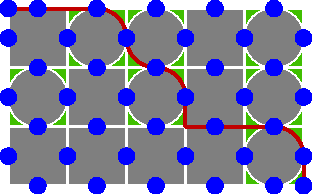
\includegraphics{sample-dots}
    }
\end{frame}

\begin{frame}
    \frametitle{\problemtitle}
    \begin{block}{Solution 1: Dijkstra}
        \begin{itemize}
            \item<+-> Turn the map into a graph,
            \begin{itemize}
                \item straight edges are $10~\text{m}$, and
                \item round edges are $5\pi~\text{m}$.
            \end{itemize}
            \item<+-> Running Dijkstra takes $\mathcal O(n \log n)$ time ($n = w \cdot h$).
        \end{itemize}
    \end{block}
    \begin{block}{Solution 2: Dynamic Programming}<3->
        \begin{itemize}
            \item<+-> For every blue vertex (left-to-right, then top-to-bottom), take the minimum between
            \begin{itemize}
                \item going straight across (right or down) and
                \item going across a corner (right-and-down or down-and-right).
            \end{itemize}
            \item<+-> This takes $\mathcal O(n)$ time ($n = w \cdot h$).
        \end{itemize}
    \end{block}
    \solvestats
\end{frame}
